\chapter{Baselines}

This chapter details the baseline forecasting models implemented to benchmark the proposed graph-based architectures. To rigorously isolate the value of relational and inter-product data, strong local baselines that rely solely on a product's own historical demand and deterministic calendar features are established. Two distinct neural network architectures were evaluated: a Long Short-Term Memory (LSTM) network, representing a standard recurrent approach to sequence modeling, and a Time-Distributed Multilayer Perceptron (MLP), representing a feed-forward approach. Before detailing the specific architecture and feature engineering of each model, this chapter first outlines the shared experimental protocol, chronological data partitioning, and evaluation metrics applied uniformly across all forecasting methods in this study.

\section{Common Training Protocol and Model Selection}
\label{subsec:training_strategies}
All forecasting models in this study used the same experimental protocol for both baseline and proposed approaches. This protocol ensured that performance differences among models reflected their ability to represent data rather than handling, optimizing, or evaluating data differently. Details of the protocol are given once and applied uniformly unless otherwise noted; only the architecture and a small number of hyperparameters specific to the architecture vary among the models. Training and evaluation for each item series used a setup that ordered the time chronologically. For each item series, the available observations were split into three segments: a training period, a validation period, and a final test period. During the training and selection of models, this final test period was completely unseen and used solely for the final recursive forecasting evaluation. This setup preserves the order of the demand series and avoids the leakage of future observations.
Before training begins, the target demand values are scaled using a min-max scaler fitted only to the training segment; this same scaler is then applied to both the validation and test segments. Exogenous variables are processed in the same way: the exogenous scaler is fitted to the training period and used to transform data in the validation and test periods. After preprocessing, both the training and validation datasets were converted into fixed-length input sequences using the selected lookback windows, and loaders were created without shuffling to preserve the temporal structure of the samples. Each model starts with its own fixed architecture but is trained using a common optimization scheme. The models used the Adam family optimizer to minimize the mean squared error (MSE). For recurrent models based on LSTM, the learning rate scheduler reduces the learning rate when the validation loss plateaus, so refinement can continue after the initial learning phase. Feed forward models based on MLPs use a fixed learning rate and do not use a scheduler; a lower base learning rate already leads to stable convergence, so annealing is not needed. 

\subsection{Chronological Data Partitioning}
\label{subsec:chronological_data_partitioning}

The total number of days of the available daily demand histories for each item in the store was 761 days. These were the days between January 23, 2021, and February 22, 2023. The number of days in the final test set was predetermined using a specific business rule. This rule stated that the models would need to predict the exact 153 days (which corresponds to approximately five months) into the future during the time frame from September 23, 2022, through February 22, 2023. Therefore, there were 608 days (between January 23, 2021, and September 22, 2022) of historical information that could be used for training and/or validating the models.

To differentiate between selecting optimal models with respect to model parameters (hyperparameters), model parameter tuning, and early stopping, all of the history after the 153-day test set was split into a 547-day training set (between January 23, 2021, and July 23, 2022) and a 61-day validation set (between July 24, 2022, and September 22, 2022). There were many reasons why a 61-day validation period ( approximately two months) was chosen. For example, choosing an appropriate amount of time to validate against will provide a long enough time span to evaluate the stability of the loss functions over various day-of-the-week and month-ending cycles. Choosing a validation cycle that is too short may introduce "background" noise into the evaluation, which is undesirable. Conversely, choosing a validation cycle that is too large will provide less than ideal signals for the model's loss function, particularly when evaluating early stopping.

This segmentation allows the use of as much continuous history as possible for training. A training window of greater than one year is extremely beneficial in retail settings. The training window of 547 days was longer than a full calendar year (365 days). Therefore, the models were trained to recognize all of the yearly holidays/promotions/seasonal transitions at least once, that is, all of the major events in the peak season associated with Black Friday and Christmas 2021. Additionally, because the training window overlaps six months with the testing window, there will be almost six months in which both windows have similar structures to train against. It is critical to describe the portion of the year that each section represents in terms of its potential impact on model selection. The validation window (July 24 to September 22, 2022) is characterized as a quiet/low promotional period that falls near the end of the summer/back-to-school season. Therefore, the validation window did not include any major retail peaks. In contrast, the test window (from September 23, 2022, to February 22, 2023) includes the entire fourth-quarter peak season. The test window includes major retail holidays, Thanksgiving, Black Friday, Christmas, and New Year, and extends through February 2023. The models were therefore validated using a relatively stable environment but were evaluated during some of the most unstable and economically valuable periods in retail. Although this creates an imbalance in terms of how the model is trained versus how it is tested, both environments represent a version of a previously observed peak season. As such, the models were exposed to all versions of these holiday demand patterns prior to their reoccurrence in the test period.

\subsection{Model Selection: Best Validation Loss}
\label{subsec:best_validation_loss}

To choose the optimal model checkpoint, a well-known validation-based method was employed to select the best-performing model based on minimum validation loss. The validation loss was computed using the validation dataset at the end of each training epoch. The set of model parameter values was updated and saved as the best checkpoint whenever an improvement in the validation loss was observed. Once a defined number of consecutive epochs passed without improvement in the validation loss (as determined by the early stopping patience parameter), training was terminated.

This method ensures the selection of the most generalized model relative to the validation portion of the dataset, based on the Mean Squared Error (MSE) criterion:
$$\theta^{*} = \arg\min_{\theta_e} \mathcal{L}_{val}(\theta_e)$$


where $\theta_e$ represents the model parameters at the conclusion of epoch e, and $\mathcal{L}_{val}$ is the loss in the validation set. Choosing a checkpoint where the validation loss is minimized provides simple yet reliable protection against overfitting to the training segment. Consequently, this ensures that the final weights are optimized for unseen data prior to the final evaluation.

\section{Recursive Multi-Step Forecasting }

\label{sec:multi_step_forecasting}

As each of the forecasting models used in this study was designed to produce a prediction that was only one time step into the future, generating forecasts over the full testing horizon of multiple time steps required the use of an autoregressive recursive rollout strategy. When making the final evaluations of the unseen test dataset, the model produced predictions sequentially. Each prediction was made by considering its previously computed prediction(s), scaling them appropriately, and adding them to the input window to compute the next prediction.

Let $L$ represent the length of the look-back window and $H$ represent the number of periods into the future that is used to make a forecast. Then, at any point in the future $t \in [1,H]$, the model is provided with an input tensor containing the most recently available $L$ target values along with their corresponding exogenous features.

The process of performing recursive inference is done in a very structured way so that temporal data do not leak through:
\begin{enumerate}
\item \textit{\textbf{Initialization}} : The input window is initialized with the final $L$ scaled target values from the validation period and the associated historical exogenous features.

\item \textbf{One-Step Forecasting} : The model makes a one-step-ahead forecast based upon the current state of the input window. It produces a single scalar forecast $\hat{y}_t$ in the scaled domain[cite: 2, 4].

\item \textbf{Inverse Scaling} : The scaled forecast $\hat{y}_t$ is converted back into its original units and added to a running buffer of all prior historical target values.

\item {\textbf{Advance Window}} : The input window is shifted one step further into the future. One element is discarded and replaced with a newly created prediction.
\end{enumerate}
A critical issue in recursively forecasting is how to track and update exogenous features for each subsequent forecasting step. As part of the experimental design, a distinction is made between static and dynamic exogenous variables, which are defined as follows:

\paragraph{Static Exogenous Variables} -

Variables whose future values are predetermined and therefore known without error at some point in the future (e.g., day of the week, month, holiday flag) are termed static. These static variables do not require processing or updating during any of the forecasting steps because their values can be determined directly from the calendar. Thus, when determining whether to include static variables in the input window for forecasting step $t + 1$, the desired values are simply looked up from the calendar and added to the bottom row of the input window before a new forecast is computed.

\paragraph{Dynamic Exogenous Variables} -

In contrast, variables that are directly dependent on a target variable (e.g., rolling mean and lagged variables) are referred to as dynamic. Dynamic variables cannot be preprocessed against ground truth data to avoid data leakage[ 2]. Therefore, they must be recalculated at each forecasting step[ 2, 4].

To clarify this point, consider the recursive forecasting algorithm. As described above, after each forecasting step, the model has access to a running buffer containing a mix of unscaled historical target values and unscaled target values that were predicted recently. For the next forecasting step($t+1)$,

\begin{itemize}
    \item Lagged features (e.g., $lag\_k$) are extracted directly from the buffer at position $-k$[cite: 2, 4].
    \item Rolling statistics (e.g., $rolling\_mean\_w$) are calculated by averaging the last $w$ elements of the unscaled buffer[cite: 2, 4]. 
\end{itemize}

After recalculation, these new dynamic values were scaled using the fitted exogenous scaler and added to the input window. This ensures that for all forecasting steps within the test horizon, the model uses only its previously generated forecasts to dynamically update the target-dependent features.

\subsection{Evaluation Metrics}
\label{subsec:evaluation_metrics}

A wide variety of evaluation metrics were used to measure and compare the forecasting models' predictive performance on data that they had never seen before, that is, the test horizon. N is defined as the total number of forecasted time periods in the test horizon, $y_{t}$ as the true or "ground truth" value of demand at time t, and $\hat{y}_{t}$ as the value predicted by the model. The following metrics were computed for each item-store series:

\paragraph{Root Mean Squared Error (RMSE)}

The RMSE is an indicator of the standard deviation of the errors generated by the model. Because it squares the errors before averaging, it heavily penalizes large deviations from the true demand, making it a critical metric for retail operations, where large forecasting errors can lead to severe stockouts or overstock situations.
\[
\text{RMSE} = \sqrt{\frac{1}{N}\sum_{t=1}^{N}(y_t - \hat{y}_t)^2}
\]

\paragraph{Mean Absolute Error (MAE)}
MAE provides a linear measure of the average magnitude of the errors, regardless of their direction. It is more robust to outliers than the RMSE and provides an easily interpretable measure of the average unit deviation.
\[
\text{MAE} = \frac{1}{N}\sum_{t=1}^{N}|y_t - \hat{y}_t|
\]

\paragraph{Mean Bias Error (Bias)}
Bias measures the systematic tendency of the model to either over-forecast or under-forecast the target variable. A positive bias indicates an overestimation of demand, whereas a negative bias indicates underestimation.
\[
\text{Bias} = \frac{1}{N}\sum_{t=1}^{N}(\hat{y}_t - y_t)
\]

\paragraph{Prediction of Change in Direction (POCID)}
While magnitude-based errors (RMSE, MAE) are important, it is also highly valuable to know whether a model accurately predicts the \textit{trend} or the direction of demand changes. POCID calculates the percentage of time steps at which the model correctly anticipates whether the demand will increase or decrease relative to the previous step.
\[
\text{POCID} = \frac{100}{N-1} \sum_{t=2}^{N} I\big((y_t - y_{t-1}) \cdot (\hat{y}_t - \hat{y}_{t-1}) > 0 \big)
\]
where $I(\cdot)$ is the indicator function that returns 1 if the condition is true and 0 otherwise.



\section{LSTM}


The LSTM Baseline was designed to be a local sequence-to-one forecasting model with the focus being the temporal characteristics of one item—time series per store. Unlike global forecasting models that share parameters across many items, this local forecasting model learned from an individual item's historical time-series data and its engineered covariates. Therefore, this is a good reference point to measure the additional value or insight that graph-based Forecasting Models will add over the insights provided by the historical demand data and engineered covariates of the target item.

For each product--store pair, the original demand series is first divided into training, validation, and test segments. The target variable was scaled using a min-max transformation fitted only on the training segment, and the same fitted scaler was then applied to the validation and test periods. The same logic was applied to the exogenous variables, ensuring that information from the validation or test periods was not used to fit the preprocessing transformations.

The forecasting model processes a fixed-size window of previous observations as an input. Each training example comprised a sequence of length $L$, where every time step included the historical target value alongside any available exogenous feature vectors. Specifically, the historical target sequence is defined as
\begin{equation}
    [y_{t-L}, y_{t-L+1}, \dots, y_{t-1}],
    \label{eq:input_target_sequence}
\end{equation}
where $y_t$ represents the value to be predicted in the future. When exogenous variables are used, they are concatenated with the target value at each time step. This process yields an input tensor of shape $(\text{batch\_size}, L, 1+p)$, where $p$ is the number of exogenous variables. 

Consequently, the temporal model (i.e., the LSTM) uses two different types of information during processing: the autoregressive history of previously recorded product demand values and either deterministic or calculated calendar-based covariates. Programming-wise, this sequence generation process is handled within a custom class that appropriately aligns the target sequence with its corresponding feature sequence prior to producing a combined input/target pair for training purposes.

The neural architecture was deliberately designed to be basic. It includes one LSTM Block, followed by a Dropout Layer and finally a Linear Output Layer. The LSTM takes sequential inputs in a chronologically ordered manner and generates a hidden representation at each time step but retains only the representation generated from the last time step because it represents a one-step-ahead forecast. After passing the hidden representation of the last time step through dropout, it passes through a linear layer that converts the hidden state into a single scalar value representing the predicted demand:
\[
\hat{y}_t = W h_{t-1}^{(LSTM)} + b.
\]
\begin{comment}
    

Thus, the implemented model has the same form as the architectural flow diagram below:

\begin{align*}
\text{Input Sequence}\rightarrow &\text{LSTM}\\ 
\rightarrow& \text{last Hidden State}\\
\rightarrow & \text{(dropout if } >0\\ 
\rightarrow& \text{ Linear Layer}\\
\rightarrow& \hat{\mathbf{y}}_t.\\
\end{align*}
\end{comment}

The \texttt{LSTM} class implements this architecture with the recurrent layers set to \texttt{batch\_first=True}, selecting only the last LSTM outputs and producing a single-dimensional prediction through a linear layer at the end.

In contrast to training the model as a one-step-ahead predictor, the model is run recursively in the testing phase to produce an overall multi-step forecast across the full forecasting horizon. The recursive process begins by taking the last available valid window of data, predicting the next value of demand, appending that prediction to the input history to generate future predictions, and then using that updated sequence to make subsequent predictions. This process continues to do so until all required test period forecasts are produced. Thus, after the initial forecast step(s), the model learns from its previous predictions instead of simply learning from historical demand observations. The recursive nature of the prediction mechanism is implemented within the inference routines, as each predicted value is utilized as part of a "rolling" input sequence to generate additional predictions.. 

Therefore, the architecture can be interpreted as an autoregressive LSTM with exogenous inputs. Its main purpose in this dissertation is to provide a strong sequential baseline: it can model nonlinear temporal dependencies in the target series, incorporate calendar and holiday effects, and generate multi-step forecasts through recursive simulations. However, it does not explicitly use the relational information between products. Consequently, any improvement obtained by graph-based models can be interpreted as evidence that inter-product similarity or dependency structures provide useful information beyond the target product’s temporal history and engineered covariates.

\begin{figure}[h!]
    \centering
    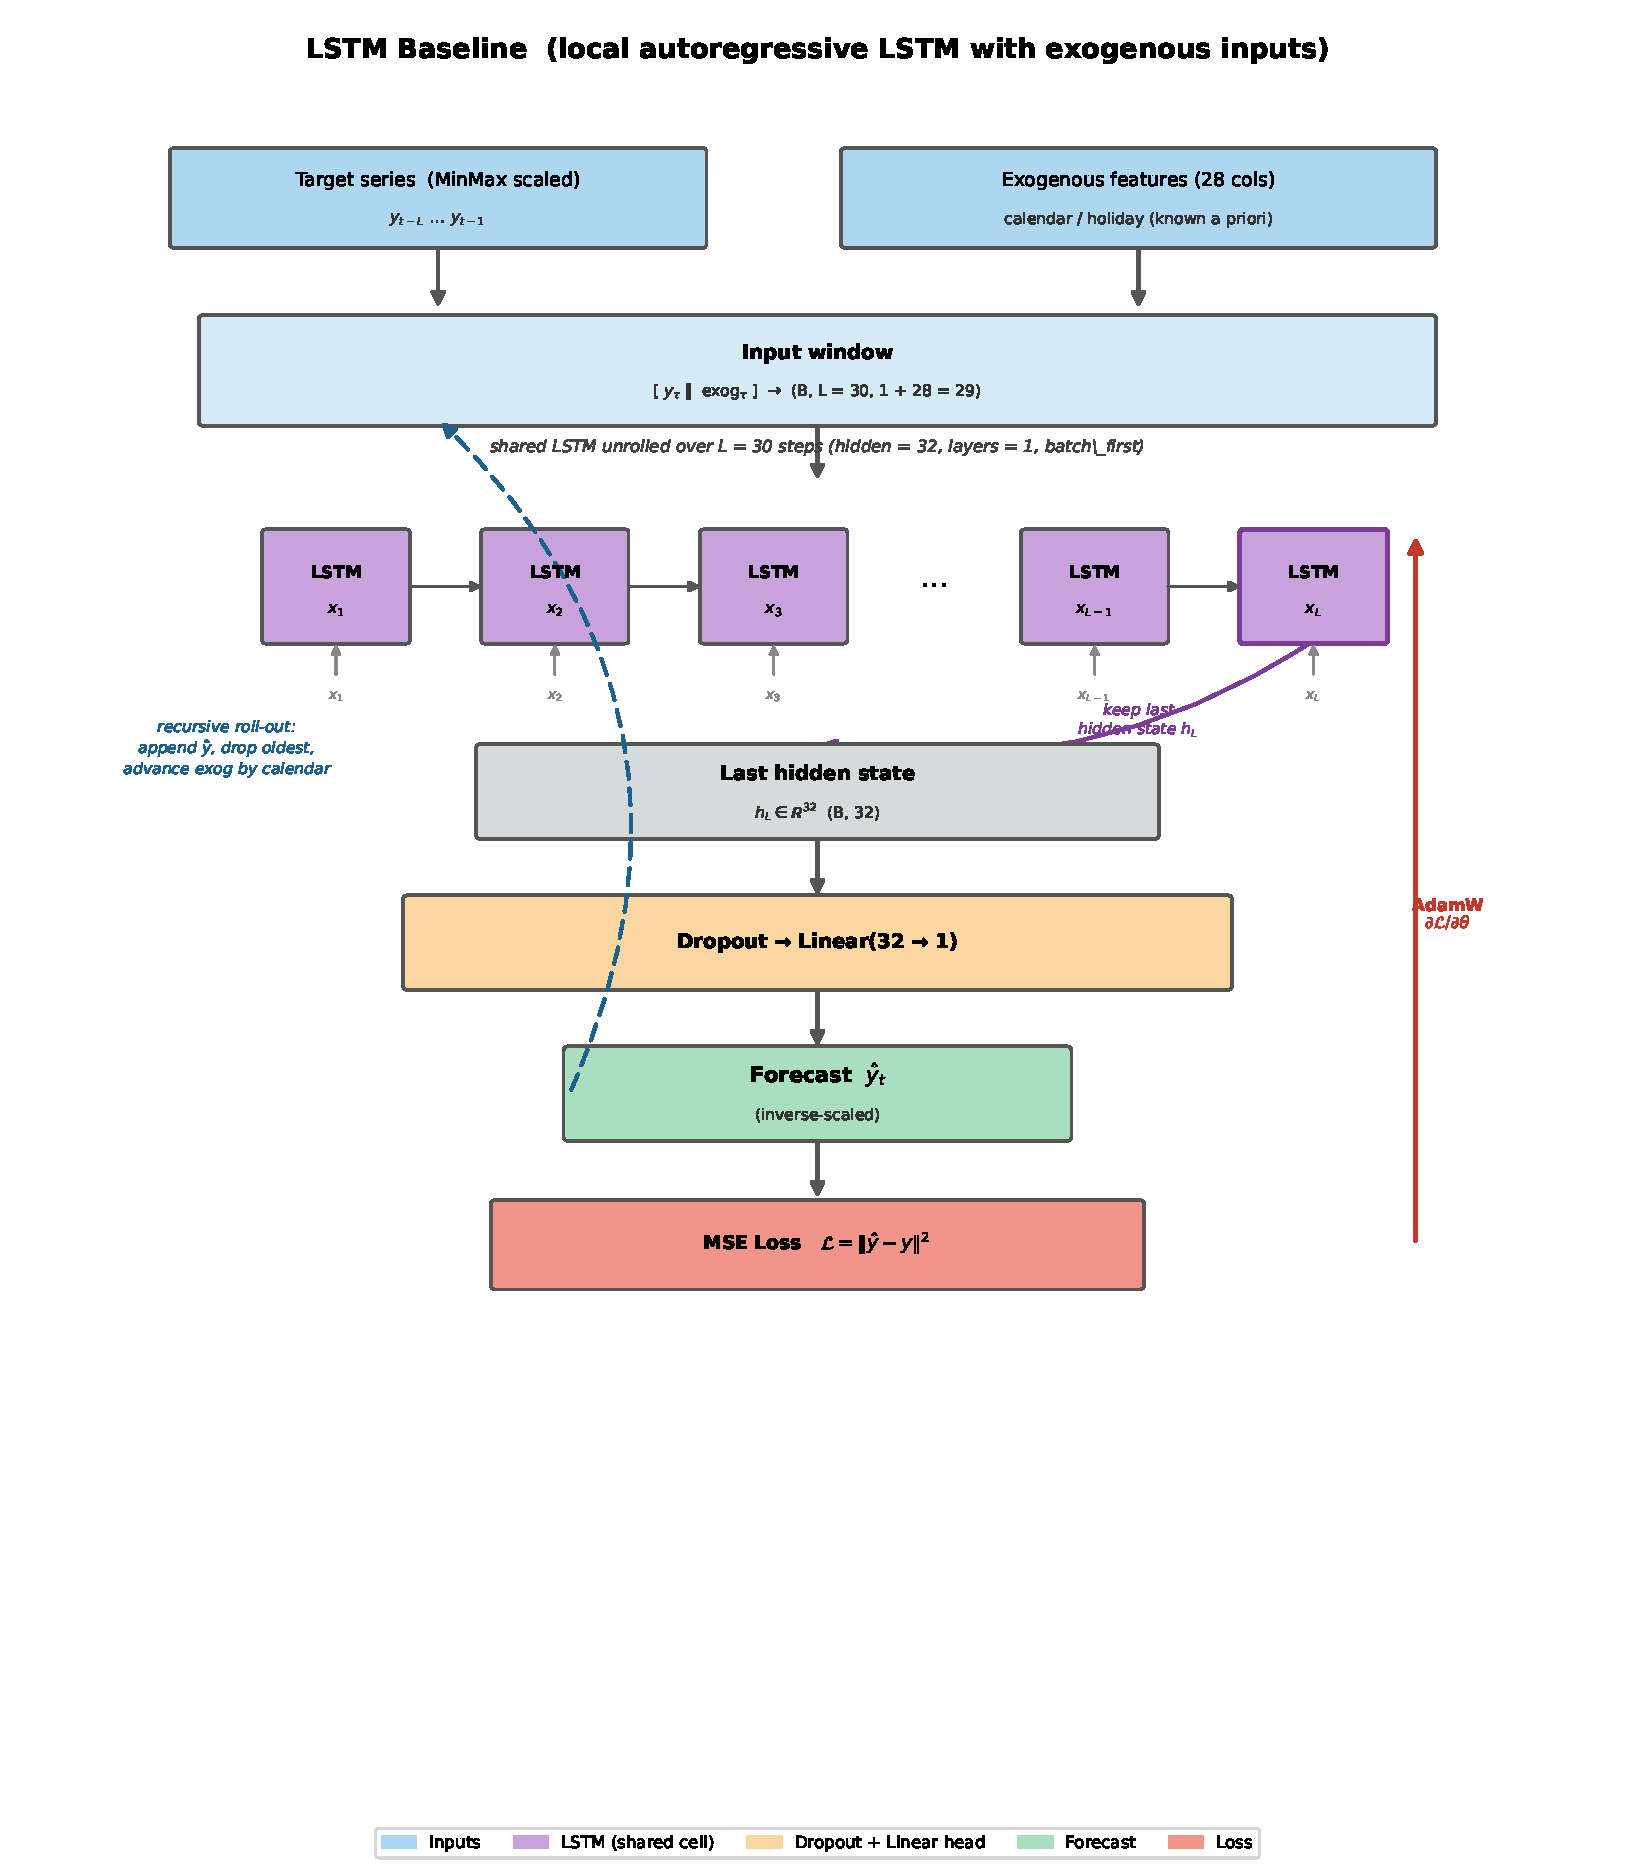
\includegraphics[width=1\linewidth]{figures/lstm_baseline_architecture.pdf}
    \caption{Local autoregressive LSTM with exogenous inputs. The MinMax-scaled target series and 28 calendar/holiday features were concatenated into an input window of length \(L=30\) and fed step-by-step through a shared single-layer LSTM (hidden size 32). The final hidden state \(\mathbf{h}_L\in\mathbb{R}^{B\times 32}\) is passed through a Dropout + Linear head to produce a one-step-ahead forecast \(\hat{y}_t\), trained end-to-end with MSE loss via AdamW. Multi-step forecasts are generated via recursive roll-out, appending each prediction as the next autoregressive input while advancing exogenous features by calendar.}
    \label{fig:placeholder}
\end{figure}
\section{Hyperparameters Chosen} 
\label {sec:lstm_hyper_parameters_chosen}

The LSTMs were implemented according to a predetermined set of architectural and optimization hyperparameter configurations. Owing to the nature of the model being used as a controlled sequential benchmark, the selected hyper-configuration represents a relatively basic architecture while limiting the model capacity so that it can effectively detect short-term non-linear relationships within the demand series.

The input sequence length or look-back window was set to $L = 30$ s. Therefore, each prediction was based on the last 30 time steps of the target series and the corresponding exogenous input variables. As such, the model will have access to nearly one month’s worth of historical demand information, including typical monthly cycles, payday impacts, and repetitive weekly patterns observed in retail-related data. The resultant input dimensionality is then $d_{\text{input}} = 1 + p$ where the first term represents the lagged target demand variable and $p$ represents the number of additional exogenous input variables included in the model.

A single LSTM layer with 32 hidden units was used in the final baseline architecture. A single recurrent layer was determined to be optimal for keeping the baseline as compact as possible while minimizing the potential for overfitting. This is particularly important because the model is trained locally for each item-store series rather than globally for all items. An internal representation capacity of 32 hidden units is considered to be of moderate complexity while maintaining a low number of trainable parameters.
Mini-batches of 32 samples were used for training. This sample size was chosen to provide a balance between stable gradient estimates and computational efficiency.

During both the training and validation periods, the mean squared error (MSE) loss function was employed. MSE was adopted for two complementary reasons: from an optimization standpoint, the squared-error objective is smooth and differentiable, providing well-behaved gradients for the AdamW optimizer and corresponding to the maximum-likelihood solution under the assumption of approximately Gaussian forecast errors, making it a standard and tractable choice for training the LSTM. From an operational standpoint, relative to a linear loss such as MAE, MSE penalizes large forecast errors disproportionately more than small errors because large errors are associated with the most severe stockout and overstock outcomes \ref{subsec:evaluation_metrics}, while small errors are comparatively inconsequential for inventory decisions. This property better aligns the training objectives with the severity of forecasting errors in a retail setting. However, MSE treats over- and under-forecasting of equal magnitude identically, whereas the underlying operational costs of these two error types — lost sales versus holding and markdown costs — are not necessarily symmetric. The MSE was nonetheless retained for this baseline configuration to keep the training objective standard and directly comparable across the architectures evaluated in this study, leaving asymmetric or quantile-based loss formulations, such as those used in quantile-output architectures such as ASG-RNN (\ref{sec:pathb-asg-rnn}), as a candidate refinement for future work.
The selected LSTM hyperparameters are listed in Table \ref{tab:lstm_hyperparameters}.

\begin{table}[H]
\centering
\caption{Base LSTM hyperparameter configuration.}
\label{tab:lstm_hyperparameters}
\begin{tabular}{ll}
\hline
\textbf{Hyperparameter} & \textbf{Chosen value} \\
\hline
Lookback window ($L$) & 30 observations \\
Batch size & 32 \\
Hidden size & 32 \\
Number of LSTM layers & 1 \\
Dropout & 0.0 \\
Optimizer & AdamW \\
Learning rate & 0.001 \\
Maximum epochs & 1000 \\
Early stopping patience & 100 epochs \\
Loss function & MSELoss \\
Learning-rate scheduler & ReduceLROnPlateau ($\times 0.5$ on plateau) \\
\hline
\end{tabular}
\end{table}



This configuration defines a local autoregressive LSTM with an exogenous input. Its role is not to exhaustively maximize predictive performance through extensive hyperparameter tuning but rather to provide a transparent and reproducible neural baseline against which the proposed graph-based forecasting approaches can be compared.



\subsection{Feature Engineering}
\label{subsec:lstm_feature_engineering}

The LSTM baseline was trained using both historical target demand and a set of engineered exogenous variables. The objective of this feature engineering step is to provide the model with contextual information that may explain systematic variations in demand that are not fully captured by the raw autoregressive sequence alone. In particular, the selected features aim to represent short-term temporal dependence, weekly and monthly calendar effects, and demand changes around relevant holidays and special dates.

For each item--store series, the input at each time step is composed of the scaled target value and the corresponding exogenous feature vector. Therefore, the model input dimensionality is defined as
\[
d_{\text{input}} = 1 + p,
\]
where the first component corresponds to the historical demand value, and \(p\) denotes the number of exogenous variables. In the implemented configuration, the exogenous variables were generated before model training and then split into training, validation, and test segments consistent with the target series. The exogenous scaler is fitted only during the training period and then applied to the validation and test periods, avoiding the use of future information in the preprocessing stage.

The selected features were grouped into four main categories. The first group consists of basic calendar-position variables, namely, \texttt{day\_of\_week}, \texttt{day\_of\_month}, \texttt{week\_of\_year}, \texttt{week\_of\_month}, \texttt{month}, and \texttt{quarter}. These variables provide the model with information about the position of each observation within the weekly, monthly, quarterly, and annual cycles. This is particularly relevant in retail demand forecasting, as customer behavior may vary systematically across weekdays, month boundaries, and seasonal periods.

The second group contains binary calendar indicators, such as \texttt{is\_weekend}, \texttt{is\_monday}, \texttt{is\_friday}, \texttt{is\_month\_start}, \texttt{is\_month\_end}, \texttt{is\_quarter\_start}, and \texttt{is\_quarter\_end}. These features allow the model to identify specific positions in the calendar that may be associated with recurring demand. For example, weekends may reflect different shopping patterns from weekdays, whereas the beginning or end of a month may capture changes associated with salary cycles, household restocking, or operational planning periods.

The final group represents holiday- and event-related effects. This includes general holiday indicators such as \texttt{is\_holiday}, specific events such as \texttt{is\_thanksgiving}, \texttt{is\_black\_friday}, \texttt{is\_christmas}, \texttt{is\_christmas\_eve}, and \texttt{is\_new\_year\_eve}, and pre- and post-holiday proximity indicators.
\[
\texttt{is\_pre\_holiday\_1},\ 
\texttt{is\_pre\_holiday\_2},\ 
\texttt{is\_pre\_holiday\_3},\ 
\texttt{is\_pre\_holiday\_7},
\]
\[
\texttt{is\_post\_holiday\_1},\ 
\texttt{is\_post\_holiday\_2},\ 
\texttt{is\_post\_holiday\_3},\ 
\texttt{is\_post\_holiday\_7}.
\]
These variables are included because retail demand is often affected not only by the holiday itself but also by the days immediately before and after it. For instance, demand may increase before major holidays owing to stockpiling behavior and decrease afterwards owing to temporary saturation. The \texttt{is\_bridge\_day} feature further captures days between holidays and weekends, which may also alter regular purchasing behavior.

The key characteristic of this final feature set is that it balances the trade-off between "explanatory richness" (i.e., providing enough detail so as to provide accurate predictions) and "parsimony" (i.e., keeping the number of features low to keep them simple). As such, it incorporates only those features that are either already known prior to running the algorithm from a knowledge perspective (e.g., based on an established calendar) or those that could easily be created from previously observed demand data. Features such as rolling means were considered in developing the feature set; however, they were ultimately determined not to be part of the base configuration. By doing so, the base case remains relatively straightforward and avoids creating smoothed versions of the target variable (which may contain some degree of duplication with respect to the explicitly lagged variables and LSTM's "look back window"). Additionally, avoiding the use of rolling averages reduced the potential ambiguity associated with recursively inferring multiple time steps into the future, where any future target-dependent features that need to be generated would have to be generated as if they were based on past predictions rather than actual values.

To properly treat lag-based features during recursive inference, after each prediction, the predicted value was added to the historical record of demand and then used to update the exogenously defined lag-based input variables for all subsequent steps. This process ensured that while internal predictions were utilized within the multistep forecasting process, this was done in a manner consistent with how the LSTM baseline itself processes information.Specifically, once the test period began, the model utilized prior predictions whenever possible to generate future auto-regressive inputs.

Overall, the engineered features incorporated into this version of the LSTM baseline made it significantly more informative than it would otherwise have been under the circumstances, that is, in comparison to what would have occurred had it been run as simply a univariate, recurrent model. However, similar to the baseline model, the current version of the LSTM baseline remains local to each item-store series. However, it allows for forecasts of individual items to depend on the calendar structure, recent memory of demand for individual items, and holiday-related impacts on demand for individual items. Consequently, this makes for a better and more appropriate benchmark against which to measure whether graph-based models offer additional predictive value beyond what is available through temporal and calendar-related information.

\section{Time-Distributed MLP}

Time-distributed Multilayer Perceptrons (TimeDistributedMLPs) are used as feed-forward forecasting models with a fixed window size of history as an input to generate a forecasted value for the next step in time. Similar to LSTMs, Time Distributed Multilayers can be trained separately per item/store combination using the same input information; however, similar to other non-recurrent models, Time Distributed Multilayers do not have any recurrent connections, gates, or memory states. Each time step of the input window is processed by a shared multilayer perceptron (MLP) (encoder), and all hidden representations produced from processing each time step are aggregated.

The number of time steps to use for the input window (\(L\)) and the number of inputs at each time step (\(C\)) are denoted by these two parameters, respectively.

Let \(L\) denote the lookback window length and \(C\) denote the number of input channels at each time step. In this setting,
\[
C = 1 + p,
\]
where the first channel corresponds to the historical target demand, and \(p\) is the number of exogenous variables. Therefore, each input sample is represented as
\[
\mathbf{X}_t \in \mathbb{R}^{L \times C}.
\]

Rather than flattening the entire temporal window into a single vector of dimension \(L \cdot C\), the TimeDistributedMLP applies the same feedforward network to each time step:
\[
\mathbf{h}_{t-j} = f_{\theta}(\mathbf{x}_{t-j}), 
\qquad j = 1,\ldots,L,
\]
where \(\mathbf{x}_{t-j} \in \mathbb{R}^{C}\) is the feature vector associated with one time step, and \(f_{\theta}\) is a shared MLP encoder. This weight sharing implies that the same nonlinear transformation is applied across all positions in the lookback window.

Each hidden representation is computed using fully connected layers with nonlinear activation and dropout regularization:
\[
\mathbf{h}^{(1)}_{t-j} = \phi(W^{(1)}\mathbf{x}_{t-j} + b^{(1)}),
\]
\[
\mathbf{h}^{(l)}_{t-j} = \phi(W^{(l)}\mathbf{h}^{(l-1)}_{t-j} + b^{(l)}).
\]

After all the time steps were encoded, the model summarized the temporal window using two complementary representations. The first is the hidden vector of the most recent time step,
\[
\mathbf{h}_{last} = \mathbf{h}_{t-1},
\]
which preserves information from the most recently observed demand state. The second is the mean-pooled representation over the full lookback window,
\[
\bar{\mathbf{h}} = \frac{1}{L}\sum_{j=1}^{L}\mathbf{h}_{t-j},
\]
This provides a global summary of the recent historical context.

These two vectors were concatenated.
\[
\mathbf{c}_t = [\mathbf{h}_{last} \, || \, \bar{\mathbf{h}}],
\]
and passed through a final linear layer to obtain a one-step-ahead forecast:
\[
\hat{y}_{t} = W_o \mathbf{c}_t + b_o.
\]

In the implemented architecture, the model outputs a tensor of the following shape:
\[
\hat{\mathbf{Y}}_t \in \mathbb{R}^{1 \times 1},
\]
corresponding to a single-step prediction of the target demand variable. Therefore, forecasts over longer horizons are produced recursively: after each prediction, the input window is advanced by one step, and the predicted value is inserted into the history used for subsequent forecasts.

\begin{comment}
    
The overall architecture can be summarized as follows:
\[
\text{Input window }(L \times C)
\rightarrow
\text{shared timestep MLP}
\rightarrow
\text{last-step representation + mean pooling}
\rightarrow
\text{output layer}
\rightarrow
\text{one-step forecast}.
\]
\end{comment}
This baseline provides a useful comparison with the LSTM because it tests whether nonlinear transformations of per-timestep demand and exogenous features, combined with a simple temporal aggregation mechanism, are sufficient for forecasting. While the LSTM learns sequential dependencies through recurrent hidden states, the TimeDistributedMLP relies on shared feed-forward encodings and a compact summary of the look-back window. Consequently, it remains simpler and faster to train than recurrent architectures while retaining some temporal information through the explicit use of the most recent hidden state and the average historical context. However, because it does not recursively model temporal transitions inside the network, it may be less capable of capturing complex ordered dependencies than an LSTM. Consistent with the fixed-rate training protocol described in Section~\ref{subsec:training_strategies}, the TimeDistributedMLP is trained at a constant learning rate without annealing; its shallower, non-recurrent structure already converges stably under the base optimizer configuration, and thus, no learning-rate scheduler is applied.


\subsection{Hyperparameters Chosen}
\label{subsec:mlp_hyperparameters_chosen}

The Time-Distributed MLP baseline was implemented as a simple feed-forward neural network that used a fixed training configuration. The network has two fully connected hidden layers (s) with 128 units in the first hidden layer and 64 units in the second (hidden) layer. In this way, the network is sufficiently complex to find nonlinear relationships between the input window and additional engineered exogenous information about the environment that will affect future demand. Simultaneously, it is less complex than other forms of neural networks, such as RNNs and GNNs. To prevent overfitting of the model during the training process, a dropout ratio of 0.2 was added.

The model was trained using batches of 32 observations for each iteration. Training with smaller batches can lead to unstable gradients and longer computation times, whereas larger batches provide better gradient estimates but may require larger memory allocations. The initial learning rate was set to \(0.001\) and the maximum allowed number of iterations was set to 1000. These parameters should be viewed as upper bounds on the training time.

AdamW was used as the optimizer along with a weight decay factor of \(10^{-3}\). Weight decay helps to add some form of regularization to the model, which limits the overfitting of the model.
The loss function used for the main configuration was the mean squared error, as follows:
\[
    \mathcal{L}_{MSE} =
    \frac{1}{n}\sum_{i=1}^{n}(y_i - \hat{y}_i)^2.
\]
This objective penalizes larger forecasting errors more strongly, which is appropriate in the retail forecasting context, where large deviations may have a greater operational impact.


\begin{table}[H]
\centering
\caption{Base MLP hyperparameter configuration.}
\label{tab:mlp_hyperparameters}
\begin{tabular}{ll}
\hline
\textbf{Hyperparameter} & \textbf{Chosen value} \\
\hline
Batch size & 32 \\
Hidden layers & $(128, 64)$ \\
Activation function & ReLU \\
Dropout & 0.2 \\
Optimizer & AdamW \\
Learning rate & 0.001 \\
Weight decay & $10^{-3}$ \\
Maximum epochs & 1000 \\
Early stopping patience & 100 \\
Loss function & MSELoss \\
\hline
\end{tabular}
\end{table}

Overall, the selected hyperparameters defined a controlled, nonlinear baseline. The goal was not to create an excessively complex model but rather to provide a reliable benchmark capable of learning from lagged target values and engineered exogenous variables before comparing them with recurrent and graph-based forecasting architectures.
\section{Feature Engineering}

\label{subsec:mlp_feature_engineering}

The Time-Distributed MLP baseline was trained on historical target demand and a set of exogenously generated features. The primary purpose of this feature engineering task was to enable the model to have explicit access to both temporal and contextual information that could be used to explain systematic variations in demand. This is particularly relevant for the MLP, because, like many feed-forward networks, MLP's are unable to remember anything about previous inputs owing to their lack of an internal hidden state. Therefore, all temporal relationships are inferred by the model when the input vector has been flattened. For every item-store pair, an input sample consists of the same look-back window size (L) as the scaled target values along with the exogenous feature vectors associated with those time steps. Thus, if the look-back window has length \(L\), the input dimensionality of the model can be defined  model as

\[ d_{\text{input}} = L(1 + p) \]
where the first element of each time step is the historical demand value, and \(p\) represents the number of exogenous features. The exogenous features were created prior to fitting the models and then split into training, validation, and test segments in synchronization with the target series. All scaling applied to these features was fit during the training phase and then applied to both the validation and test phases to prevent using any information available after the fact within the pre-processing stage.

The selected features were grouped into four main categories. The first group consists of cyclical calendar-position variables.
\[
\begin{split}
&\texttt{dow\_sin},\quad \texttt{dow\_cos},\\
&\texttt{doy\_sin},\quad \texttt{doy\_cos},\\
&\texttt{dom\_sin},\quad \texttt{dom\_cos},\\
&\texttt{wom\_sin},\quad \texttt{wom\_cos},\\
&\texttt{month\_sin},\quad \texttt{month\_cos},\\
&\texttt{quarter\_sin},\quad \texttt{quarter\_cos},\\
&\texttt{woy\_sin},\quad \texttt{woy\_cos}.
\end{split}
\]
These variables encode the position of each observation within the weekly, monthly, quarterly, and annual cycles. Sine and cosine transformations were used instead of simple ordinal values because they preserved the cyclical nature of time. For example, the transition from Sunday to Monday, December to January, or the last week of the year to the first week of the following year should be interpreted as a short temporal distance rather than a large numerical jump. By representing calendar positions using paired sine and cosine components, the MLP can learn smoother periodic patterns across multiple temporal cycles.

The second group contains binary calendar boundary indicators:
\[
\texttt{is\_month\_start},\quad
\texttt{is\_month\_end},\quad
\texttt{is\_quarter\_start},\quad
\texttt{is\_quarter\_end}.
\]
These features allow the model to identify specific positions in the calendar that may be associated with recurring demand. For example, the beginning or end of a month may capture changes related to purchasing behavior, replenishment routines, reporting cycles, salary effects, or other operational patterns. Similarly, quarterly boundaries may reflect changes associated with planning, inventory management, or business reporting periods.

The third group is composed of short-term demand-level features.
\[
\texttt{rolling\_mean\_excl\_7}.
\]
This variable provides a smoothed signal of recent demand intensity based on historical observations, excluding the current target value. As a result, it can be used during training without directly leaking the predicted value. This feature helps the MLP identify whether a product is currently in a higher- or lower-demand regime, complementing the raw lagged target values already included in the fixed input window. This is especially useful for a feed-forward model because it does not update a recurrent memory state as it processes the sequence.

The fourth group represents holiday- and event-related effects. This includes the general holiday indicator
\[
\texttt{is\_holiday},
\]
as well as specific retail-relevant events.
\[
\begin{gathered}
\texttt{is\_thanksgiving},\quad
\texttt{is\_black\_friday},\quad
\texttt{is\_christmas},\\
\texttt{is\_christmas\_eve},\quad
\texttt{is\_new\_year\_eve}.
\end{gathered}
\]
The feature
\[
\texttt{is\_bridge\_day}
\]
is also included to identify days between holidays and weekends. These variables were included because retail demand can change sharply on specific dates. Major holidays and shopping events may produce demand spikes, whereas bridge days may deviate from normal weekday behavior due to altered shopping routines, store visits, or household planning patterns.

Therefore, the final feature set was designed to provide the MLP with explicit information about the calendar position, structural calendar boundaries, recent demand intensity, and special retail events. Compared with the LSTM baseline, the MLP uses cyclical sine--cosine encodings more extensively because it does not process the input sequence through a recurrent hidden state. These encodings help the model interpret recurring temporal patterns from a flattened representation of the input window.

During recursive inference, target-dependent features require special treatment because future observed demand values are no longer available. In particular, the rolling mean feature must be updated using the available demand history, which progressively includes previous predictions once the test horizon begins. After each forecast, the predicted value was appended to the demand history and used to construct the input features for the subsequent steps. This ensures that the multistep forecasting procedure remains consistent with the recursive nature of the Time-Distributed MLP baseline.

\begin{figure}[h!]
    \centering
    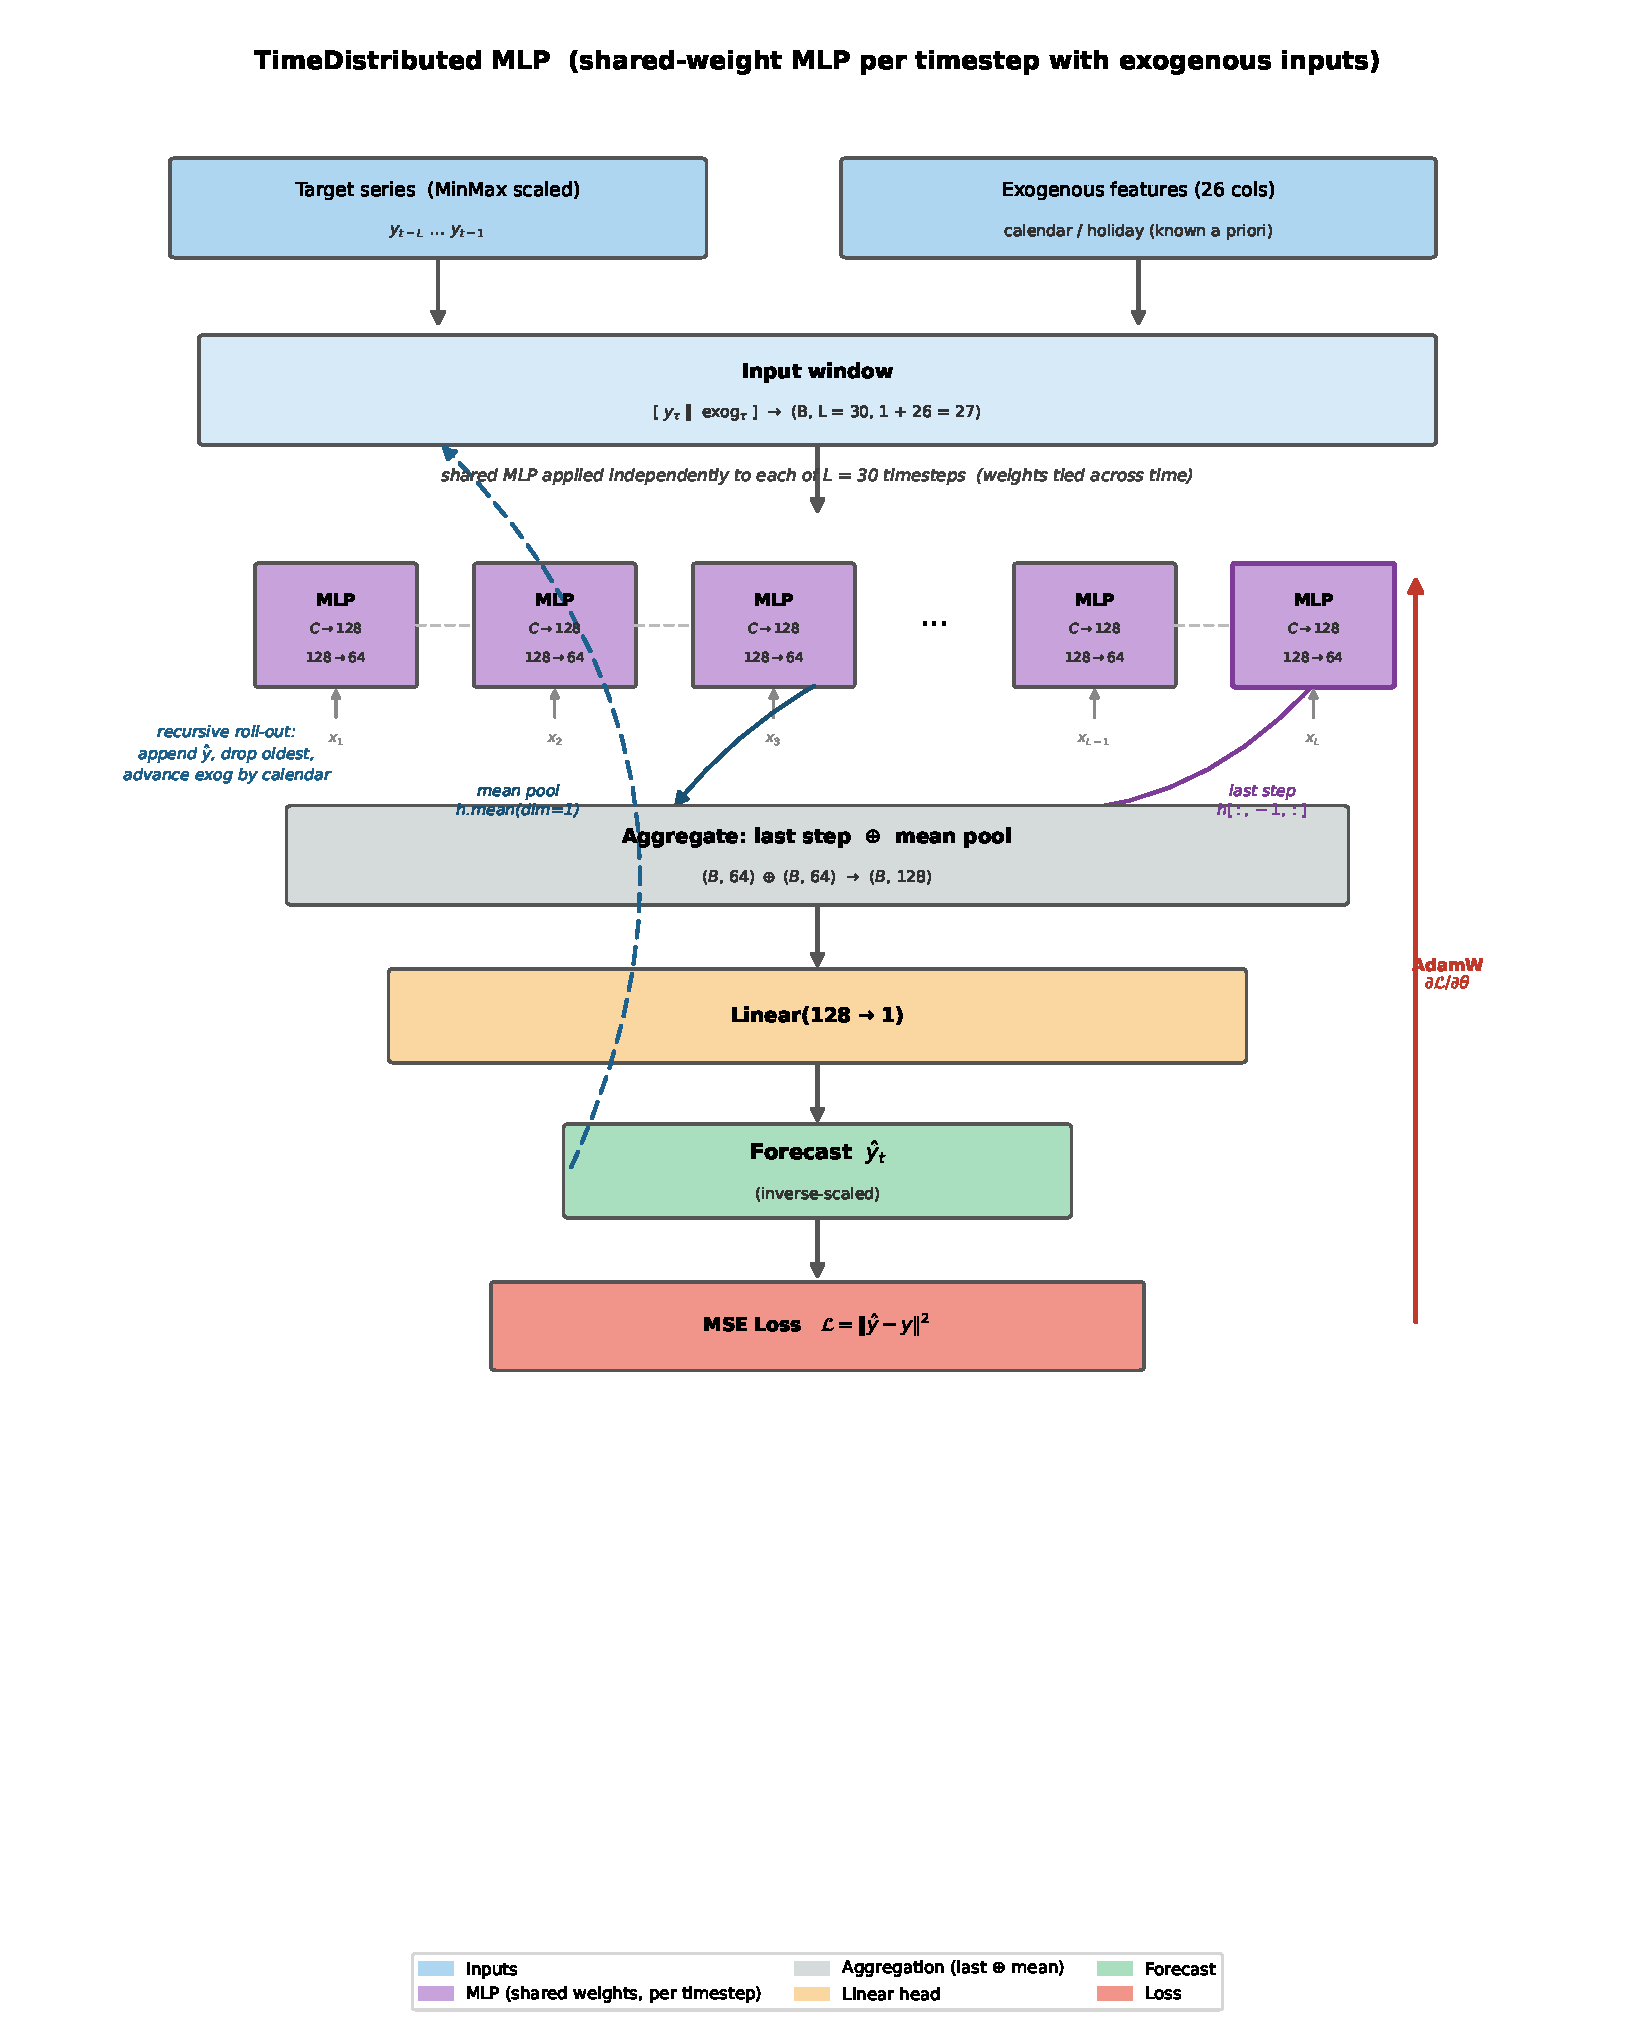
\includegraphics[width=1\linewidth]{figures/tdmlp_architecture.pdf}
    \caption{Example model architecture (the local autoregressive Time-Distributed MLP baseline). Although the training and evaluation protocols are shared across all models, the internal architecture differs for each model. Here, at each step $\tau$, the concatenated input $[y_\tau \parallel \text{exog}_\tau] \in \mathbb{R}^{27}$ is passed through the same two-layer MLP ($C \to 128 \to 64$, ReLU + Dropout), producing a sequence of hidden representations $h \in \mathbb{R}^{B \times L \times 64}$. Two complementary signals are then extracted: the last step $h[:, -1, :]$ (recency) and the temporal mean $\bar{h}$ (global context), which are concatenated into $(B, 128)$ and projected by a single linear ($128 \to 1$) head to yield the one-step-ahead forecast $\hat{y}_t$. Training minimises MSE via AdamW; multi-step forecasts are generated by recursive roll-out, feeding each $\hat{y}_t$ back as the next autoregressive input while advancing the exogenous features by calendar.}
    \label{fig:placeholder}
\end{figure}

